\chapter{Testing}
\label{chp:testing} 

\section{Testplan}

\section{Results}

\subsection{Simulations}

\begin{figure}[p]
	\centering
	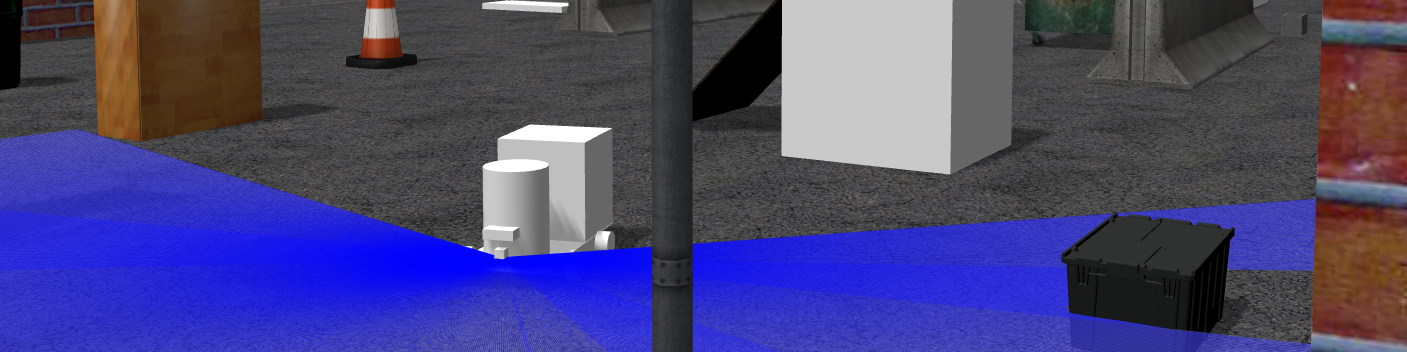
\includegraphics[width=1\textwidth]{gazebo2_cropped}
	\caption{The ''Asphalt'' world in Gazebo. }
	\label{fig:Incorrect_lc_detection}
\end{figure}

\begin{figure}[p]
	\centering
	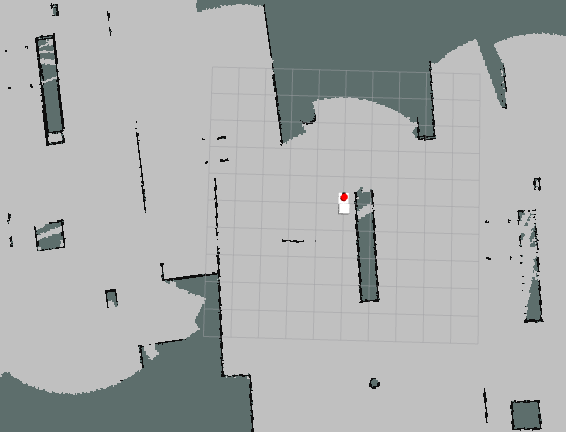
\includegraphics[width=1\textwidth]{Incorrect_lc_detection_cropped}
	\caption{An example of incorrect map merging. This case occurred in the ''Asphalt'' world simulated in Gazebo.}
	\label{fig:Incorrect_lc_detection}
\end{figure}

\begin{figure}[p]
	\centering
	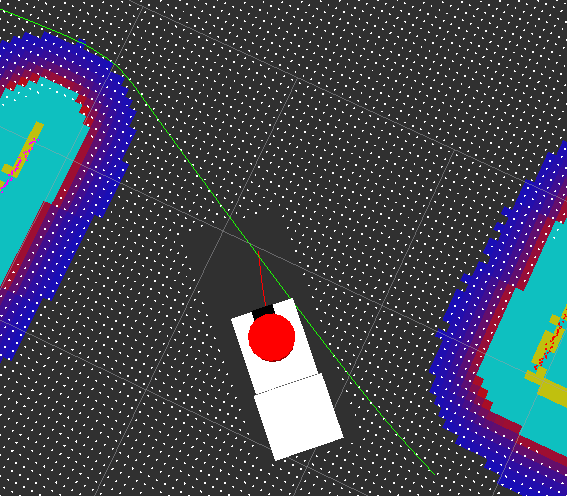
\includegraphics[width=1\textwidth]{planning_big_footprint_cropped}
	\caption{Nodes and topics for motion control. }
	\label{fig:big_footprint}
\end{figure}

\subsection{Live Testing}

\subsubsection{Safety Features}

\subsubsection{Loop Closure Detection}

\subsubsection{Multi Session Mapping}

\subsubsection{Navigating an Obstacle Course}

\begin{figure}
	\centering
	\begin{subfigure}[b]{0.46\textwidth}
		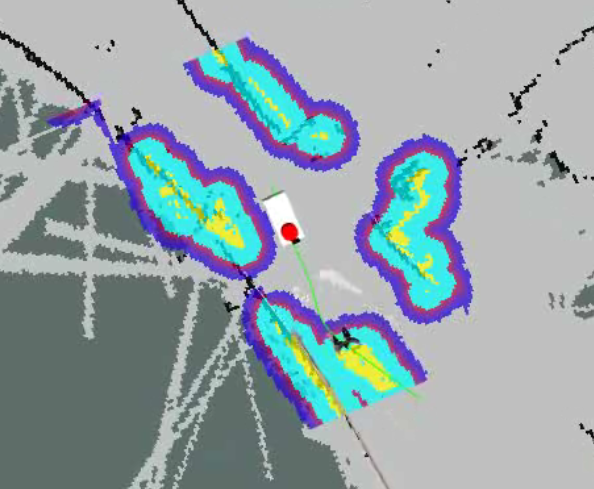
\includegraphics[width=\textwidth]{obstructed_plan}
		\caption{A person has moved into the path of the robot.}
		\label{fig:obstructed_plan}
	\end{subfigure}
	\begin{subfigure}[b]{0.472\textwidth}
		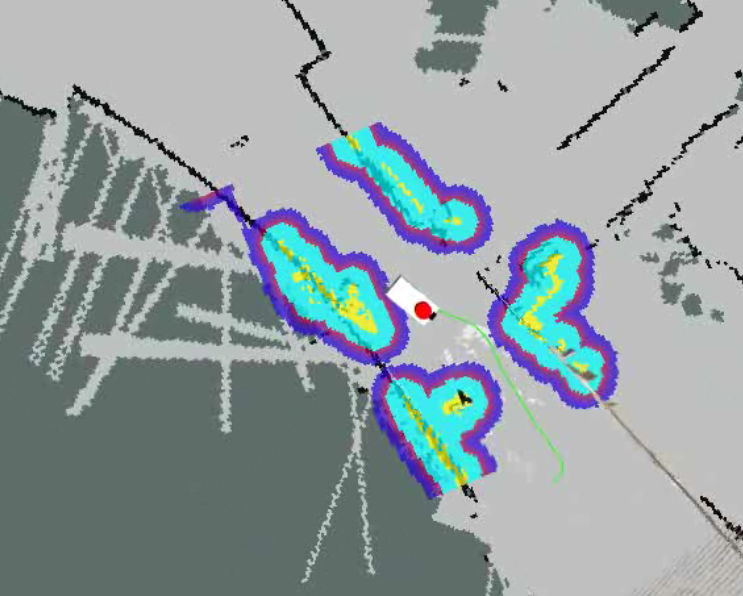
\includegraphics[width=\textwidth]{corrected_plan}
		\caption{A new path is planned, avoiding the new obstacle.}
		\label{fig:corrected_plan}
	\end{subfigure}
    \caption{Moving obstacle avoidance. The local cost map, shown as coloured spots on the occupancy grid, is based on real-time sensor data. }
\end{figure}

\subsubsection{Avoiding Moving Obstacles}






\section{Discussion}